\documentclass{article}
\usepackage[a4paper, total={6in, 10in}]{geometry}
%\setlength{\parskip}{0.01cm plus4mm minus3mm}

\usepackage{multicol}
\usepackage{enumitem}

\usepackage{listings}
\usepackage{xparse}

\usepackage[superscript,biblabel]{cite}
\usepackage{graphicx}
\usepackage{hyperref}
\usepackage{caption}

\usepackage{blindtext}
\usepackage{dirtree}

\usepackage{xcolor}
\colorlet{cBlue}{blue!80}
\colorlet{cPurple}{blue!40!red}
\colorlet{cRed}{red!60}

\NewDocumentCommand{\codeword}{v}{
    \texttt{\textcolor{cBlue}{#1}}
}

\NewDocumentCommand{\cmd}{v}{
    \textit{\textcolor{cPurple}{#1}}
}

% Styles stolen from https://www.overleaf.com/learn/latex/Code_listing
\definecolor{codegreen}{rgb}{0,0.6,0}
\definecolor{codegray}{rgb}{0.5,0.5,0.5}
\definecolor{codepurple}{rgb}{0.58,0,0.82}
\definecolor{backcolour}{rgb}{0.95,0.95,0.92}

\lstdefinestyle{mystyle}{
    backgroundcolor=\color{backcolour},
    commentstyle=\color{codegreen},
    keywordstyle=\color{magenta},
    numberstyle=\tiny\color{codegray},
    stringstyle=\color{codepurple},
    basicstyle=\ttfamily\footnotesize,
    breakatwhitespace=false,
    breaklines=true,
    captionpos=b,
    keepspaces=true,
    numbers=left,
    numbersep=5pt,
    showspaces=false,
    showstringspaces=false,
    showtabs=false,
    tabsize=2
}

\lstset{style=mystyle}

\title{\Huge Coursework 3: Genshin Impact Simulator}
\author{William Bradford Larcombe \small (K21003008) \\ Pawel Makles \small (K21002534)}
\date{\small Created: 1st March 2021 \\ Last Modified: 2nd March 2021}

\begin{document}
    % Cover Page
    \maketitle
    \vfill
    \centering 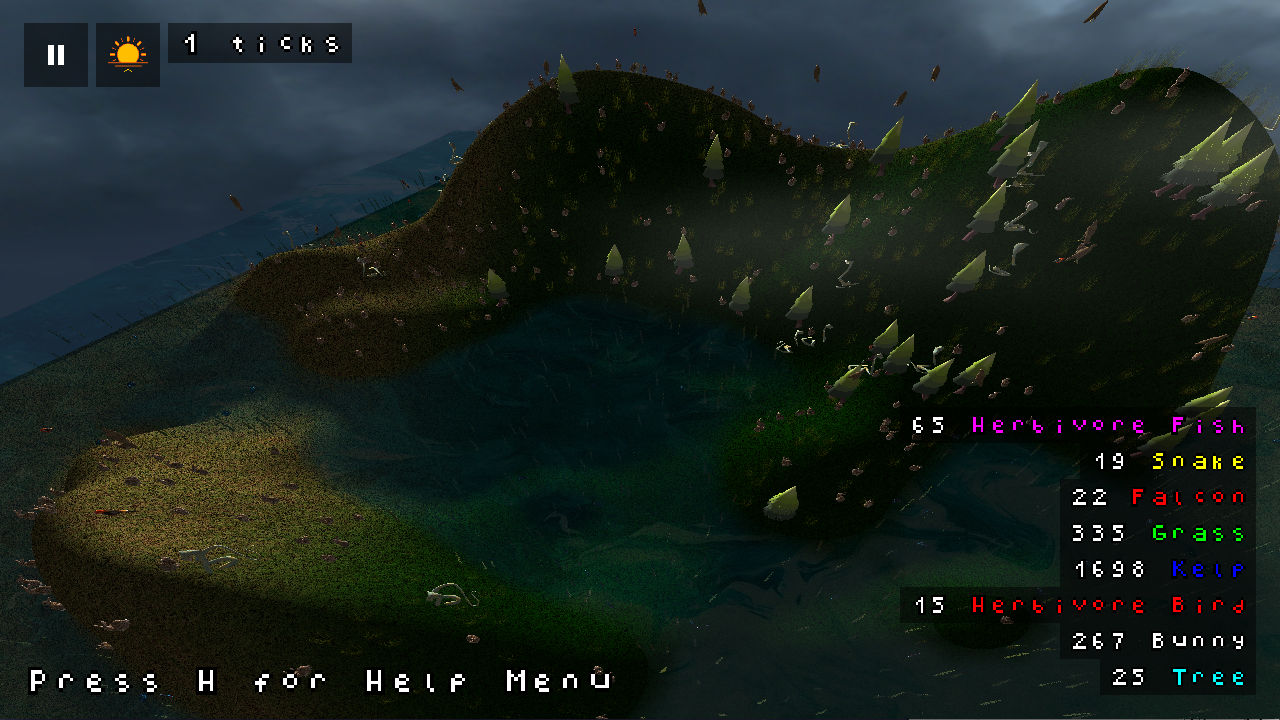
\includegraphics[width=\textwidth]{../screenshot.png}
    
    \newpage

    \begin{multicols}{2}
        \section{The Simulation}

        \subsection{Species List}

        \subsection{Species Interactions}
        
        \section{Challenge Tasks}

        % Layered simulation and interactions between them
        \subsection{Multi-layered Simulation (Foliage + Aerial)}
        % this is one of the provided challenge tasks

        % Could talk about implementation of AI
        \subsection{Brain and Behaviour Model}

        % Graphics Section
        \subsection{3D Rendered Simuation}

        % other provided tasks that we haven't done:
        % \subsection{Weather}
        % \subsection{Disease}

    \end{multicols}

    \newpage

    % IGNORE OLD CONTENT:
    % WILL BE TOUCHING
    \begin{thebibliography}{9}
        \bibitem{beastman}
        Brand New Animal Wiki. Beastman \\
        \url{https://brand-new-animal.fandom.com/wiki/Beastman}
        \bibitem{animacity}
        Brand New Animal Wiki. Animacity \\
        \url{https://brand-new-animal.fandom.com/wiki/Anima_City}
        \bibitem{marie}
        Brand New Animal Wiki. Marie Itami \\
        \url{https://brand-new-animal.fandom.com/wiki/Marie_Itami}
        \bibitem{bna}
        IMDb. BNA (TV Mini Series 2020) \\
        \url{https://www.imdb.com/title/tt12013558/}
        \bibitem{utopia}
        IMDb. Utopia (TV Series 2013-2014) \\
        \url{https://www.imdb.com/title/tt2384811/}
        \bibitem{excalidraw}
        Excalidraw. \\
        \url{https://excalidraw.com/}
        \bibitem{bluej}
        GitHub. maven-bluej / BlueJ.java \\
        \url{https://github.com/KCLOSS/maven-bluej/blob/master/BlueJ.java}
        \bibitem{river-map}
        Google Maps. Jezioro Świerklaniec, Poland \\
        \url{https://www.google.com/maps/@50.4293559,18.9742453,16.12z}
        \bibitem{common-weights}
        PDF. Set of average weights for furniture, appliances and other items \url{https://democracy.york.gov.uk/documents/s2116/Annex\%20C\%20REcycling\%20Report\%20frnweights2005.pdf}
        \bibitem{pyrocynical}
        YouTube. The best (and worst) show you haven't seen \\ \url{https://youtu.be/PFx2QM0Z8Qo}
        \bibitem{bluej-issue}
        GitHub. BlueJ Bug Reproductions (wip) \\ \url{https://github.com/insertish/bluej-bug-demo}
        \bibitem{font}
        Fontsource. VT323 \\ \url{https://fontsource.org/fonts/vt323}

        \textbf{\\ References in code.}

        \bibitem{code-ref-1}
        \codeword{Ansi.java} StackOverflow. How to print color in console using System.out.println? \\
        \url{https://stackoverflow.com/a/5762502}
        \bibitem{code-ref-2}
        \codeword{LocalisedIO.java} StackOverflow. What is the equivalent of Regex-replace-with-function-evaluation in Java 7? \url{https://stackoverflow.com/a/27359491}
        \bibitem{code-ref-3}
        \codeword{JTerminalFrame.java} How to detect a key press in Java \\
        \url{https://stackoverflow.com/a/21970006}
        \bibitem{code-ref-4}
        \codeword{JTerminalView.java} How to "do something" on Swing component resizing? \\
        \url{https://stackoverflow.com/a/8917978}
        \bibitem{code-ref-5}
        \codeword{JTerminalView.java} Java Documentation. Font Concepts \\
        \url{https://docs.oracle.com/javase/tutorial/2d/text/fontconcepts.html}
        \bibitem{code-ref-6}
        \codeword{JTerminalView.java} Java Documentation. Java Thread Primitive Deprecation \url{https://docs.oracle.com/javase/1.5.0/docs/guide/misc/threadPrimitiveDeprecation.html}
        \bibitem{code-ref-7}
        \codeword{JTerminalView.java} StackOverflow. Drawing Canvas on JFrame \\
        \url{https://stackoverflow.com/a/17922749}
        \bibitem{code-ref-8}
        \codeword{TerminalEmulator.java} StackOverflow. Passing values between 2 threads without intrrrupting each other \url{https://stackoverflow.com/a/23413506}

        \textbf{\\ Libraries used:}
        \bibitem{library-1}
        \cmd{com.moandjiezana.toml} \url{https://github.com/mwanji/toml4j}
        \bibitem{library-2}
        \cmd{commons-io} \url{https://commons.apache.org/proper/commons-io}
        \bibitem{library-3}
        \cmd{kuusisto.tinysound} (fork by DrogoniEntity) \url{https://github.com/DrogoniEntity/TinySound}
        \bibitem{library-4}
        \cmd{com.projectdarkstar.ext.jorbis} \\
        \url{https://search.maven.org/artifact/com.projectdarkstar.ext.jorbis/jorbis}
        \bibitem{library-5}
        \cmd{com.googlecode.soundlibs.tritonus-share} \\
        \url{https://search.maven.org/artifact/com.googlecode.soundlibs/tritonus-share/0.3.7.4/bundle}
        \bibitem{library-6}
        \cmd{com.googlecode.soundlibs.vorbisspi} \\
        \url{https://search.maven.org/artifact/com.googlecode.soundlibs/vorbisspi/1.0.3.3/bundle}

        \textbf{\\ Sounds used:}
        \bibitem{sound-money-bag}
        Freesound. "Money Bag" by PhilSavlem (licensed under CC0) \\
        \url{https://freesound.org/people/PhilSavlem/sounds/338260/}
        \bibitem{sound-waves-1}
        Freesound. "bay of fundy 01.flac" by tim.kahn (licensed CC BY 3.0) \\
        \url{https://freesound.org/people/tim.kahn/sounds/127569/}
        \bibitem{sound-waves-2}
        Freesound. "bay of fundy 02.flac" by tim.kahn (licensed CC BY 3.0) \\
        \url{https://freesound.org/people/tim.kahn/sounds/127568/}
        \bibitem{sound-bgm-1}
        Freesound. "2020-03-17 Lofi Trip Hop" by Doctor\_Dreamchip (licensed CC BY 3.0) \\
        \url{https://freesound.org/people/Doctor_Dreamchip/sounds/511279/}
        \bibitem{sound-bgm-2}
        Freesound. "Remix of GioMilko Freesound \#417960.flac" by Timbre (licensed CC BY-NC 3.0) \\
        \url{https://freesound.org/people/Timbre/sounds/418692/}
        \bibitem{sound-bgm-3}
        Freesound. "loopable Lo-fied remix of Tenshi\_Mixer freesound \#585947.flac" by Timbre (licensed CC BY-NC 3.0) \url{https://freesound.org/people/Timbre/sounds/586988/}
        \bibitem{sound-forest-birds}
        Freesound. "Birds In The Forest" by BurghRecords (licensed under CC0) \\
        \url{https://freesound.org/people/BurghRecords/sounds/456123/}
        \bibitem{sound-worm-hole}
        Freesound. "Bed of entanglement" by CosmicD (licensed CC BY 3.0) \\
        \url{https://freesound.org/people/CosmicD/sounds/133007/}
        \bibitem{sound-city-1}
        Freesound. "VOC\_150325-0973-1\_HK\_citywalk.wav" by kevp888 (licensed CC BY 3.0) \\
        \url{https://freesound.org/people/kevp888/sounds/440973/}
        \bibitem{sound-city-2}
        Freesound. "VOC\_150325-0972\_HK\_citywalk.wav" by kevp888 (licensed CC BY 3.0) \\
        \url{https://freesound.org/people/kevp888/sounds/440974/}

    \end{thebibliography}
    
    \newpage

    % Appendix
    \captionsetup{justification=centering,margin=3cm}
    \begin{figure}
        \centering
        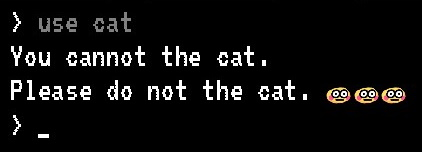
\includegraphics[width=\textwidth]{images/emoji.jpg}
        \caption{Sample emoji output} \label{fig:emoji}
    \end{figure}
%     \begin{figure}
%         \centering
%         \includegraphics[width=\textwidth]{../src/main/resources/map/base.png}
%         \caption{World Map} \label{fig:map}
%     \end{figure}
%     \begin{figure}
%         \centering
%         \includegraphics[width=\textwidth]{images/runaway-raccoon-302.jpg}
%         \caption{Shot of Animacity as seen in Episode 1 at 3:02 of Brand New Animal \cite{bna}} \label{fig:runaway-raccoon}
%     \end{figure}
%     \begin{figure}
%         \centering
%         \includegraphics[width=\textwidth]{images/festival-marie.jpg}
%         \caption{Michiru Kagemori and Marie Itami pictured left to right in Episode 1 at 12:51 of Brand New Animal \cite{bna}} \label{fig:festival-marie}
%     \end{figure}
%     \begin{figure}
%         \centering
%         \includegraphics[width=\textwidth]{images/help-command.jpg}
%         \caption{Output from the help command} \label{fig:help-command}
%     \end{figure}
%     \begin{figure}
%         \centering
%         \includegraphics[width=\textwidth]{images/terminal.jpg}
%         \caption{The terminal emulator} \label{fig:terminal}
%     \end{figure}
%     \begin{figure}
%         \centering
%         \includegraphics[width=\textwidth]{images/map-ingame.jpg}
%         \caption{Output from the map command} \label{fig:map-ingame}
%     \end{figure}
%     \begin{figure}
%         \lstinputlisting[language=Java]
%         {../src/main/java/uk/insrt/coursework/zuul/events/Event.java}
%         \caption{Event.java (uk.insrt.coursework.zuul.events.Event)} \label{fig:event}
%     \end{figure}
%     \begin{figure}
%         \lstinputlisting[language=Java]
%         {../src/main/java/uk/insrt/coursework/zuul/io/IOSystem.java}
%         \caption{IOSystem.java (uk.insrt.coursework.zuul.io.IOSystem)} \label{fig:io-system}
%     \end{figure}
%     \begin{figure}
%         \lstinputlisting[language=Java]
%         {../src/main/java/uk/insrt/coursework/zuul/io/StandardIO.java}
%         \caption{StandardIO.java (uk.insrt.coursework.zuul.io.StandardIO)} \label{fig:standard-io}
%     \end{figure}
%     \begin{figure}
%         \lstinputlisting[language=Java]
%         {../src/main/java/uk/insrt/coursework/zuul/io/LocalisedIO.java}
%         \caption{LocalisedIO.java (uk.insrt.coursework.zuul.io.LocalisedIO)} \label{fig:localised-io}
%     \end{figure}
%     \begin{figure}
%         \lstinputlisting[language=Java]
%         {../src/main/java/uk/insrt/coursework/zuul/events/EventSystem.java}
%         \caption{EventSystem.java (uk.insrt.coursework.zuul.events.EventSystem)} \label{fig:event-system}
%     \end{figure}
%     \begin{figure}
%         \lstinputlisting[language=Java]
%         {../src/main/java/uk/insrt/coursework/zuul/dialogue/DialogueOption.java}
%         \caption{DialogueOption.java (uk.insrt.coursework.zuul.dialogue.DialogueOption)} \label{fig:dialogue}
%     \end{figure}
%     \begin{figure}
%         \lstinputlisting[language=Java]
%         {../src/main/java/uk/insrt/coursework/zuul/ui/EventDraw.java}
%         \caption{EventDraw.java (uk.insrt.coursework.zuul.ui.EventDraw)} \label{fig:event-draw}
%     \end{figure}
%     \begin{figure}
%         \begin{lstlisting}[language=Java]
% public<E extends Event> void addListener(Class<E> event,
%     IEventListener<E> listener) {
%     this.getList(event).add(listener);
% }\end{lstlisting}
%         \caption{Excerpt from EventSystem.java (uk.insrt.coursework.zuul.events.EventSystem)} \label{fig:generic-method}
%     \end{figure}
%     \begin{figure}
%         \begin{lstlisting}[language=Java]
% /**
%  * Get the current weight of this inventory.
%  * @return Weight (in kg)
%  */
% public double getWeight() {
%     return this
%         .items
%         .stream()
%         .mapToDouble(Entity::getWeight)
%         .sum();
% }

% /**
%  * Check if the inventory is full.
%  * @return True if the weight is greater than the max weight
%  */
% public boolean isFull() {
%     return this.getWeight() >= this.getMaxWeight();
% }

% /**
%  * Add an entity to this inventory.
%  * 
%  * There must be sufficient space for the entity.
%  * @param entity Target Entity
%  * @return Whether we successfully added the new entity.
%  */
% public boolean add(Entity entity) {
%     if (this.getWeight() + entity.getWeight() > this.maxWeight) {
%         return false;
%     }

%     this.items.add(entity);
%     return true;
% }\end{lstlisting}
%         \caption{Excerpt from Inventory.java (uk.insrt.coursework.zuul.entities.Inventory)} \label{fig:inventory}
%     \end{figure}
%     \begin{figure}
%         \begin{lstlisting}[language=Java]
% /**
%  * Write a string value to the text buffer.
%  * @param value String value to write
%  */
% public void write(String value) {
%     // Write each character sequentially.
%     for (int i=0;i<value.length();i++) {
%         char c = value.charAt(i);

%         // If we encounter an Ansi escape character, then take the
%         // substring from this point on and determine if it is a valid
%         // escape code. If it is, apply any changes before continuing.
%         if (c == '\u001B') {
%             Matcher matcher = Ansi.AnsiPattern.matcher(value.substring(i));
%             if (matcher.find()) {
%                 int v = Integer.parseInt(matcher.group(1));
%                 i += 3 + (v > 9 ? 1 : 0);

%                 if (v == 0) {
%                     this.bg = Color.BLACK;
%                     this.fg = Color.WHITE;
%                 } else if (v >= 30 && v < 38) {
%                     this.fg = Ansi.fromEscapeCode(v);
%                 } else if (v >= 40 && v < 48) {
%                     this.bg = Ansi.fromEscapeCode(v);
%                 }

%                 continue;
%             }
%         }

%         this.write(c);
%     }
% }\end{lstlisting}
%         \caption{Excerpt from TextBuffer.java (uk.insrt.coursework.zuul.ui.TextBuffer)} \label{fig:ansi-match}
%     \end{figure}
\end{document}
